\section{Introduction}
\label{intro}
\indent
For a long time past, squaric acid ($\text{H}_2\text{C}_4\text{O}_4$, also known as $\text{H}_2\text{SQ}$) has been intensely investigated  exploring  various  aspects arising from the interacting hydrogen-bonds (H-bonds). The interacting H-bonds are responsible for a wide range of phenomena observed in nature such as proton transfer processes in enzyme catalysis~\cite{mathias2007structures}, concerted proton transfers in membrane water channels~\cite{brewer2001formation,dellago2003proton} and cooperative proton tunneling in water hexamers~\cite{chen2013nature,bove2009anomalous}. Recently, hydrogen-bonded systems are being looked into plausible technological devices which exploit the H-bonds to induce electrically ordered quantum states~\cite{lengyel2019}. There have been extensive studies looking into its strong electronic (anti) ferroelectric polarizability~\cite{fjaer1980light,petersson1980phase,horiuchi2018strong,dolin2011quantum,horiuchi2008organic,horiuchi2020hydrogen}. With the recent realization of room-temperature ferroelectricity observed in one such H-bonded ferroelectrics~\cite{horiuchi2005ferroelectricity,horiuchi2012above}, there seems to be a strong possibility for future applications. Apart from the ferroelectric properties, hydrogen-bonded systems could also be used in detecting confinement to deconfinement transition~\cite{huang2017deconfinement}. Though experimentally it is maybe a challenging task to detect the deconfined charges~\cite{huang2017deconfinement} yet it would validate certain lattice gauge theories~\cite{chern2014gauge}. \\
\indent An interesting aspect of hydrogen-bonded systems is that the hydrogen ions (or protons) satisfy local constraints known as the \textit{ice-rules}. Depending on the details of the electronic structure of the material, the number of protons engaged in the \textit{ice-rules} vary. For example, for materials (such as squaric acid) with fundamental unit as a square plaquette there are two protons that are nearer and two protons farther on any given plaquette in an ice-rule state. From these ice-rules and the structural phase transition perspective, among various H-bond systems the squaric acid bears many similarities with water ice~\cite{benton2016classical}. However, the significance of squaric acid comes from the simplicity of it's quasi-2D nature and also from the \textit{squaric} geometry of $\text{C}_4\text{O}_4$ molecules.\\% And also for the three-dimensional structure of hexagonal water ice ($I_h$) similar to the squaric acid which exists as weakly coupled quasi-two-dimensional layers. \\
%\indent The crystal structure of $\text{H}_2\text{SQ}$ consists of quasi-2D layers stacked one above the other with each alternating layer shear displaced slightly along the horizontal direction (see Fig.~\ref{lattice}(a)). It is known that despite its three-dimensional structure, the material is known to manifest its quasi-two-dimensional behavior. Specifically, low values of the critical exponent for order parameter ($f_i$= 0.17 and 0.14) obtained respectively from measurements of the optical birefringence~\cite{semmingsen1974structural} and of the neutron scattering~\cite{WANGY1974}, were found to have a characteristic of a two-dimensional transition. This poses a question as to how the layers have been stacked antiferroelectrically and what might be the role of interlayer coupling. However, from the experiments of \textit{Nakashima et al}~\cite{nakashima1976raman}, we know that the interlayer interaction acts only between the hydrogen bonds of adjacent layers and is localized in the region near the H-bonds. Following this, a theory has been put forth suggesting that the interlayer coupling may be the reason for high transition temperatures, $T_c$, and for a phase transition to happen~\cite{maier1980phenomenological}.\\
\indent It may be noted that various theoretical works were mostly limited to the quasi two-dimensional nature of squaric acid~\cite{ishizuka2011quantum,chern2014gauge,vijigiri2018classical,huang2017deconfinement,ishibashi2018computational,matsushita1982cluster}. Early theories based on order-disorder transition coupled with lattice (phonon) degrees of freedom motivated in explaining the (anti)ferroelectric order for a quasi-2D layer. This was supported by the findings where low values of the critical exponent for an order parameter ($f_i$= 0.17 and 0.14) were observed using optical birefringence~\cite{semmingsen1974structural} and  neutron scattering~\cite{WANGY1974} experiments. It is also known that the nearest neighbour two-dimensional planes are found to be (anti) ferroelectrically stacked~\cite{hollander1977molecular}. Although this indicates that an interlayer coupling between the two dimensional planes must exist and be weak, yet the nature of interaction to our knowledge is still unknown.  The squaric acid exhibits a characteristic phase transition from low temperature antiferroelectric phase to a high temperature paraelectric phase of first-order. Unlike the other H-bonded counterparts like $\text{KH}_2\text{PO}_4$, the transition temperature $T_c$ is unusually high pointing towards a possible role of interlayer coupling. This therefore, necessitates to consider an interlayer coupling  between adjacent layers for a qualitative understanding of transition temperatures versus interlayer coupling. And thus from a purely theoretical (adventurous) point of view, the study of three dimensional spin models become very important in its own right. Motivated by these, we here introduce and investigate a three dimensional pseudo-spin models applicable for $\text{H}_2\text{SQ}$. \\
\indent In our endeavour to study the three dimensional characteristics of proton dynamics relevant to $\text{H}_2\text{SQ}$, we extend the two-dimensional model studies~\cite{chern2014gauge, vijigiri2018classical} to three-dimensions by considering a nearest neighbour interlayer interaction of Ising type.
In the absence of first principle study, we consider all possible types of interlayer coupling such as ferroelectric (FM), antiferroelectric (AFM) and disordered type (where some bonds are randomly chosen ferromagnetic ($J_3 < 0$) and the rest to be antiferromagnetic ($ J_3 > 0$)).  We find that various phases such as long-range  antiferroelectric phase, quantum-liquid-like intermediate phase that are found in 2D-cases \cite{vijigiri2020dipole,ishizuka2011quantum} are sensitive in different ways in each of the different type of interlayer coupling. Although there is no distinction between the AFM and FM type coupling there is a significance deviation of physical quantities when the coupling is of disordered type. Briefly, our quantum Monte Carlo results show that the extent which the long ranged antiferroelectric phase extends in temperature is qualitatively same for AFM and FM type and different for disordered type interlayer coupling. In AFM and FM cases, the intermediate quantum-liquid like state vanishes slowly as when the strength ogsurvives for small values and vanishes after certain threshold interlayer coupling. As the interlayer coupling is increased the phase transition from AFE phase to quantum liquid-like state transforms to a phase transition from AFE to conventional paraelectric phase. Interestingly, our semi-classical analysis using spin-wave approximations corroborate the findings from QMC where the spin-wave spectrum is shown to be independent of the sign (type) of the interlayer coupling. In both the cases the the spin-wave velocity acquires a finite value proportional to the magnitude of interlayer coupling. Our detailed plan of presentation is given below.\\
%Most of the theories that have been put forward were based on the order-disorder mechanism dictating the ice-rules type physics in the low-temperature monoclinic phase. It may be noted that the order-disorder mechanism could be best explained by mapping the proton system to a quantum spin system comprising pseudo-spins. Here, the protons are represented by pseudo-spin variables corresponding to a suitable quantum spin Hamiltonian. As far as $\text{H}_2\text{SQ}$ is concerned, one of the prominent models that are currently gaining significance is based on the Ising lattice-gauge theory in (2+1)~\cite{chern2014gauge,kogut} dimensions with spins located on the edges of a unit square plaquette (see Fig.~\ref{lattice}(b)). Within the model, when only the quasi-2D nature was taken into account, the material was shown to host three different phases. As indicated, they are, 1) antiferroelectric (AFE), 2) quantum liquid-like, and 3) deconfined phase. \\
%\indent Apart from the fact that in a given layer, the dipoles (molecular polarization) are antiferroelectrically ordered, it is also known that the layers were stacked antiferroelectrically~\cite{hollander1977molecular}. Due to this fact, one may believe that the interlayer interaction to be of antiferromagnetic. However, in the present work, we show that even in cases that include disorder or ferromagnet, the material could support antiferromagnetic stacked configurations provided the interlayer interaction is weak compared to the intralayer interactions. Since the distortion of lattice at the critical point also could point out the non-uniformity of the interlayer coupling. We, therefore, invoke the non-uniform nature of interlayer coupling $J_3$ in our simulations and analyze the effect of it on the quasi-2D phases. We use the pseudo-spin formalism and employ the discrete version of the path-integral continuous-time quantum Monte Carlo technique to arrive at our results~\cite{nakamura2008efficient}. To distinguish three different phases,  we estimate various quantities such as the order parameters, $P$, $\rho$, and the imaginary-time correlation function, $c_\tau$, as a function of the transverse field, $K$. %It may be noted that $c_\tau$ measures the gauge-invariant correlation when the dipole-dipole interaction is turned off. We believe that the study of interlayer coupling is important as a sufficient interlayer interaction strength could lead to concerted proton tunneling between the interlayers dictating an alternative physics. \\
\begin{figure}[t!]
%\label{lattice}
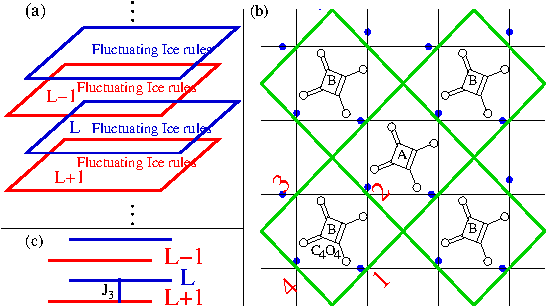
\includegraphics[width=8.8cm,height=5cm]{figures/3D_lattice.pdf}
\caption{(Color online) Schematic illustrating the detailed 3D lattice structure of $\text{H}_2\text{SQ}$. (a) Bird's eye view of $\text{H}_2\text{SQ}$ crystal lattice showing interlayers (labeled as $L-1,L,L+1$) coupled through the Ising exchange coupling $J_3$ (see (c)). (b) Schematic showing the lattice structure within a given quasi-2D layer. The small colored dots (blue) represent the protons
and while the compound $\text{C}_4\text{O}_4$ form a quasi-2D layered configuration with protons placed on the links of a dual lattice (green lines).  The local proton ordering which in the pseudospin language is $\mid \uparrow \rangle$, $\mid \downarrow \rangle$. (c) Cross-sectional view of the 3D $\text{H}_2\text{SQ}$ lattice structure. The indices $L-1, L, L+1$ correspond to $L-1^{\text{th}}, L^{\text{th}}, L+1^{\text{th}}$ layer respectively. Each square plaquette is occupied by exactly one square molecule where ice-rules are conserved by the gauge and Ising coupling constants, $J_0, J_1$.}
\label{lattice}
\end{figure}
\indent We begin by introducing the model in details in Sec. ~\ref{model} by briefly explaining the implementation details of the quantum Monte Carlo scheme.  Next in Sec.~\ref{quantities} we introduce and explain the different order parameters used to determine the presence of various phases such as global antiferroelectric phase and an intermediate quantum liquid phase. We also define imaginary-time correlation function which has been used to locate the  confined-deconfined phase transition.  In Sec. \ref{results}  we presents our results. First we discuss the effect of interlayer coupling on the spin-wave spectrum and spin wave velocity in both low and high-field limits. Next we present the resu lts of imaginary-time correlation function and obtain a qualitative understanding of the confinement-deconfinement transition as we increase the magnitude of external magnetic field. Following this, we present the antiferroelectric polarization order parameter, $P$ and ice-rule order parameter, $\rho$ (and corresponding susceptibility) versus temperature (and field) to draw the phase diagram in $T-K$ plane. Finally, we briefly present the dynamic structure factor obtained for two-dimensional layer where we argue its possible connection to the experiments.  In Sec.~\ref{discussion}, we discuss and briefly summarize our results .
%%%%%%%%%%%%%%%%%%%%%%%%%%%%%%%%%%%%%%%%%%%%%%%%%%%%%%%%%%%%%%%%%
                % Model and Method
%%%%%%%%%%%%%%%%%%%%%%%%%%%%%%%%%%%%%%%%%%%%%%%%%%%%%%%%%%%%%%%%%
